\documentclass[../main.tex]{subfiles}
\begin{document}
\chapter{Special Relativity}
\section{Basic Postulates of Relativity}
In 1862, Maxwell's equations predicted the existence of electromagnetic waves that travel in a vacuum at the \textit{speed of light}.
The speed of light $c$ is \textbf{exactly equal to}:
\[
  c = \qty{299792458}{\metre\second^{-1}} \approx \qty{3e8}{\metre\second^{-1}}
\]
\begin{remark}[Note]
  The speed of light is exactly this value because one metre is defined as the distance travelled by light in a vacuum during a time of $1/299792458$ seconds.
\end{remark}

A theory with a ``preferred velocity'' cannot be Galilean invariant.
Galilean theories can only have \textbf{relative velocities}.
In principal, a definite velocity could be acceptable, for example, sound in air also travels at a definite speed $v_{s} \approx \qty{300}{\metre\second^{-1}}$, however, this is \textbf{relative to the air} which is at rest.
So, if you move towards a sound wave with speed $v$, you would measure sound travelling at a speed $v_s + v$.
This lead us to assume that light must also be travelling in some fixed medium, this was called the \textit{ether}.

However, there was an experiments in 1881 by Michelson and Morley that effectively showed that, regardless of the velocity of the observer, you always measure light travelling at the same speed $c$.

This caused a massive crisis in physics, until, in 1905, Einstein postulated that there was no ether and two other postulates:
\begin{enumerate}
  \item The laws of physics are the same in all inertial frames -- This is the same as what Galileo postulated (\cref{galileanRelativity}) and is called the \textit{principal of relativity}.
  \item The speed of light $c$ is the same in \textbf{all inertial frames} -- This is incompatible with inertial frames being related by Galilean transformations as velocities add under Galilean transformations.
\end{enumerate}
\section{1D Lorentz Transformations}
\subsection{Derivation}
We need to change the rules for transforming between frames to ensure that the speed of light is the same in all frames.
We will start with a single spatial dimension $x$ and then build up to higher dimensions later.

Suppose we have frame $S$ with coordinates $(x, t)$ and a frame $S'$ with coordinates $(x', t')$ that moves at a constant velocity $v$ relative to $S$.

According to Galileo, the frames should be related by:
\begin{align*}
  x' &= x - vt \\
  t' &= t
\end{align*}
However, under Einsteins postulates, this is not possible as the speed of light will be different in each frame.

\subsubsection{Finding General Form}
We will start from a general relation:
\begin{align*}
  x' &= f(x, t) \\
  t' &= g(x, t)
\end{align*}
and then show that this leads to a \textit{Lorentz Transformation}.
From the first postulate, the law of inertia is still true, that is, a particle experiencing no forces moves at a constant velocity in all frames.
For such a particle:
\begin{align*}
  \text{In $S$: }& x = A + Bt \\
  \text{In $S'$: }& x' = A' + B't
\end{align*}
Transformations that achieve this are called \textit{affine transformations} which are a linear transformation composed with a translation.
Here, we will choose our frames to share a common origin, i.e. $x = t = 0 \iff x' = t' = 0$ and so $A = A' = 0$.
We can do this as we can always just shift $x$ and $x'$ by constants.
Therefore, the transformation must map all lines passing through the origin in the $(x, t)$-plane to lines passing through the origin in the $(x', t')$-planes, these are precisely linear transformations.

Thus, the transformation must have the form:
\begin{align*}
  x' &= \alpha_1x + \alpha_2t \\
  t' &= \alpha_3x + \alpha_4t
\end{align*}
where $\alpha_i$ are constants that do not depend on $x$ or $t$ but can depend on the relative velocity between frames, since it is constant.

The frame $S'$ is moving at speed $v$ in the frame $S$, but $S'$ is at rest with respect to itself, this means that $x = vt$ should map to $x' = 0$, thus:
\[
  x' = \gamma_v(x - vt)
\]
for some $\gamma_v$ that depends on the relative velocity of the frames $v$.

\subsubsection{Showing $\gamma_v = \gamma_{-v}$}
\begin{lemma}
  Where defined as above, $\gamma_v = \gamma_{-v}$.
\end{lemma}
\begin{proof}
  Consider the frames $\widetilde{S}$ and $\widetilde{S}'$ which are the frames $S$ and $S'$ where the $x$ axis is inverted in direction, that is $\widetilde{x} = -x$ and $\widetilde{x}' = -x'$.

  $S'$ moves at speed $v$ with respect to $S$ and so $\widetilde{S}'$ moves at speed $-v$ with respect to $\widetilde{S}$.
  Therefore:
  \[
    \widetilde{x}' = \gamma_{-v}(\widetilde{x} + \widetilde{t}) = \gamma_{-v}(\widetilde{x} + t)
  \]
  noting that $\widetilde{t} = t$ since time is invariant when inverting just the axis direction.

  Mapping back into the original $x$ axis:
  \[
    -x' = \gamma_{-v}(-x + vt)  \implies x' = \gamma_{-v}(x - vt)
  \]
  and so $\gamma_{v} = \gamma_{-v}$.
\end{proof}
We now define $\gamma \equiv \gamma_{v} = \gamma_{-v}$, noting that it can still depend on velocity.
\begin{remark}
  Another argument for this property is that in 3D, there is no ``preferred'' direction and so $\gamma$ can only depend on the magnitude of the velocity $v^2 = |\vec{v}|^2$ and so $\gamma_v = \gamma_{-v}$.
\end{remark}
\subsubsection{Finding Coefficients in Terms of $\gamma$}
We also require that if we boost by $v$, and then by $-v$, we should get back to the original frame.
That is, a boost by $-v$ is the inverse of a boost by $v$:
\[
  S \xrightarrow{\ v\ } S' \xrightarrow{-v\ }S'' = S
\]
First, considering the boost from $S' \to S''$:
\[
  x'' = \gamma_{-v}(x' + vt') = \gamma(x' + vt')
\]
and then for the boost from $S \to S'$:
\[
  x' = \gamma_{v}(x - vt) = \gamma(x - vt)
\]
Combining the above, we have:
\begin{align*}
  x'' &= \gamma(\gamma(x - vt) + vt') \\
      &= \gamma^2 (x - vt) + \gamma vt'
\end{align*}
We require this to just be $x$ and so:
\[
  \gamma^2 (x - vt) + \gamma vt' = x \implies t' = \gamma t + \frac{1 - \gamma^2}{\gamma v} \cdot x
\]
So we now have $t'$ and $x'$ in terms of $t$ and $x$, with $\gamma$ as the only undetermined quantity.

\subsubsection{Determining $\gamma$ Using the 2nd Postulate}
We can now use the second postulate to determine $\gamma$.
Since the speed of light needs to be the same in both frames, the light ray $x = ct$ must map to $x' = ct'$.
\[
  x' = \gamma(x - vt) = \gamma(ct - vt) = \gamma t(c - v)
\]
and
\[
  t' = \gamma t + \frac{1 - \gamma^2}{\gamma v} \cdot ct
\]
So for $x' = ct'$ to hold, we require:
\[
  \gamma t(c - v) = c\left(\gamma + \frac{1 - \gamma^2}{\gamma} \cdot \frac{c}{v}\right)t
\]
Solving the quadratic for $\gamma$, we have:
\[
  \gamma = \frac{1}{\sqrt{1 - \frac{v^2}{c^2}}}
\]
where we took the positive root to avoid reflecting the $x$ axis.
\begin{remark}
  If $v \geq c$, then we have issues so this transformation only makes sense for $v < c$.
  We will understand this restriction properly later.
\end{remark}
\begin{definition}[Lorentz Transformations]
  \textit{Lorentz Transformations} or \textit{boosts} are transformations of the form:
  \label{lorentzTransforms}
  \begin{align*}
    x' &= \gamma(x - vt) \\
    t' &= \gamma\left(t - \frac{v}{c^2} \cdot x\right)
  \end{align*}
  where $\gamma = \frac{1}{\sqrt{1 - \frac{v^2}{c^2}}}$ is the \textit{Lorentz factor}.
\end{definition}
\begin{remark}[Sanity Check]
  For velocities $v \ll c$, $\gamma \approx 1$ and $\frac{v}{c^2} \to 0$ so we recover the Galilean transformations $x' = x - vt$ and $t' = t$.
  In general, assuming that $v \ll c$ is called taking the ``non-relativistic limit''.
\end{remark}
\subsection{Addition of Velocities}
Suppose we have a particle moving at a speed $u'$ in a frame $S'$ which is moving at a speed $v$ in frame $S$.
We want to know what speed $u$ the particle moves at in the frame $S$.

To do this, we can use an inverse Lorentz transformation.
By how we derived these transformations, we see that to do the inverse transform, we just need to take $v \mapsto -v$ and so:
\[
  x = \gamma(x' + vt') \text{ and } t = \gamma\left(t' + \frac{v}{c^2}x'\right)
\]
Since the speed of the particle is constant, in $S$ $x = ut$ and in $S'$ $x' = u't'$.
Therefore:
\[
  u = \frac{x}{t} = \frac{x' + vt'}{t' + \frac{v}{c^2}x'} = \frac{\frac{x'}{t'} + v}{1 + \frac{v}{c^2}\frac{x'}{t'}} = \frac{u' + v}{1 + \frac{vu'}{c^2}}
\]
So the relativistic formula for addition of velocities is:
\[
  u = \frac{u' + v}{1 + \frac{vu'}{c^2}}
\]
\begin{remark}[Sanity Check]
  If $v, u' \ll c$, then $\frac{vu'}{c^2} \to 0$ and we just retrieve the standard addition of velocities $u = u' + v$ we would expect for Galilean transformations.
\end{remark}
Furthermore, if $|u'|$ and $|v|$ are both less than $c$, then so is $|u|$.
For example, if $u' = v = \frac{c}{2}$, then Galileo would tell us that $u = c$, whereas we now see that:
\[
  u = c \cdot \frac{\frac{1}{2} + \frac{1}{2}}{1 + \frac{1}{4}} = \frac{4}{5}c
\]
So we cannot make something travel faster than light by moving our frame towards it at a large velocity.

We also see that if $u' = v = c$, then:
\[
  u = \frac{c + c}{1 + c^2/c^2} = c
\]
so if we try to add the speed of light to itself, we get the speed of light back, which is what we wanted.
\subsection{Space-time Diagrams and Simultaneity}
The following type of diagram is called a \textit{space-time diagram}:
\begin{center}
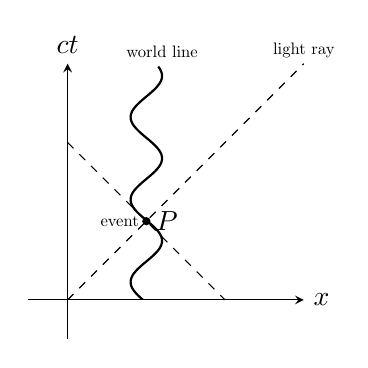
\begin{tikzpicture}[>=stealth]
  \draw[->] (-0.5, 0)  -- (3, 0) node[right] {$x$};
  \draw[->] (0, -0.5)  -- (0, 3) node[above] {$ct$};

  \node[scale=0.6, above] at (1.2, 3) {world line};
  \node[scale=0.6, above] at (3, 3) {light ray};
  \fill (1, 1) circle (1.5pt) node[right] {$P$} node[left, scale=0.6, xshift=-1] at (1, 1) {event};
  \draw[dashed] (0, 2) -- (2, 0);
  \draw[dashed] (0, 0) -- (3, 3);
  \clip (0, 0) rectangle (3, 3);
  \draw[thick, domain=0:3, smooth, samples=100, rotate=90, yshift=-1cm,xshift=-1] plot (\x,{0.2 *sin(6 *\x r)});
\end{tikzpicture}
\end{center}
\textbf{Features of a space-time diagram}:
\begin{itemize}
  \item A point $P$ on a space-time diagram is called an \textit{event} and represents a point in space and time.
  \item The trajectory of a particle through a space-time diagram is called a \textit{word line} or \textit{worldline}.
  \item The dashed lines on the diagram represent light rays emitted from the particle.
  \item Since the axes are $ct$ and $x$, rays of light must travel at $\pm\ang{45}$ as they have $x = a \pm ct$ for some constant $a$.
\end{itemize}
We can also superpose the axes for a frame $S'$ on the space-time diagram of $S$.
We can use the equations from \cref{lorentzTransforms} to find what the $t'$ and $x'$ axes are mapped to in $S$.

In the frame $S'$, the $ct'$ axis corresponds to the line $x' = 0$:
\[
  x' = 0 = \gamma(x - vt) \implies x = vt \implies ct = \frac{c}{v}x
\]
Similarly, in $S'$, the $x'$ axis corresponds to the line $t' = 0$:
\[
  t' = 0 = \gamma(t - \frac{v}{c^2} x) \implies x = \frac{c^2}{v}t \implies ct = \frac{v}{c}x
\]
So they are mapped to the lines $ct = \frac{c}{v}x$  and $ct = \frac{v}{c}x$.
Noting that $\frac{c}{v} > 1$ and $\frac{v}{c} < 1$, we can draw this onto the space-time diagram for $S$:
\begin{center}
\begin{tikzpicture}[>=stealth]
  \draw[->] (-3, 0)  -- (3, 0) node[right] {$x$};
  \draw[->] (0, -3)  -- (0, 3) node[above] {$ct$};

  \draw[dashed] (-3, 3) -- (3, -3);
  \draw[dashed] (-3, -3) -- (3, 3);

  \node at (3.3, 1.8) {$x'$};
  \node at (1.9, 3.3) {$ct'$};
  \begin{scope}[decoration={
      markings,
      mark = at position 0.91 with {\arrow{>}}
    }]
    \clip (-3, -3) rectangle (3, 3);
    \draw[rotate=15, postaction={decorate}] (-3, -3) -- (3, 3);
    \draw[rotate=-15, postaction={decorate}] (-3, -3) -- (3, 3);
  \end{scope}
\end{tikzpicture}
\end{center}
\begin{remark}[Note]
  The axes for $S'$ are always symmetric about the line $ct = x$ as $ct = \frac{c}{v}x$ and $ct = \frac{v}{c}x$ are reflections of each other in the line $ct = x$.
\end{remark}
\end{document}
